\documentclass[11pt,onecolumn,draftclsnofoot]{IEEEtran}

\usepackage[utf8]{inputenc}
\usepackage[T1]{fontenc}
\usepackage{setspace}
\usepackage{graphicx}
\usepackage{float}
\usepackage{amsmath}
\usepackage{booktabs}
\usepackage[hidelinks]{hyperref}
\onehalfspacing
\newcommand{\wordcount}{
\immediate\write18{texcount -1 -sum -merge main.tex > wordcount.txt}
\input{wordcount.txt}
}

\begin{document}

\begin{titlepage}
    \centering
    \vspace*{0.18\textheight}

    {\LARGE \bfseries Three-phase linear models outperform alternative models for scale limited Tetraselmis tetrahele growth dataset  \par}

    \vspace{2.5cm}

    {\large Zhou Yang \par}
    \vspace{0.6cm}
    {\large Imperial college London \par}
    {\large zy3425@ic.ac.uk \par}

    \vfill

\begin{center}
Word count: \wordcount
\end{center}

    {\large \today \par}
\end{titlepage}

\setcounter{page}{1}

\begin{abstract}
Population growth models affect not only goodness of fit, but also the biological interpretation of different phases. Inadequate model may fail to distinguish these phases clearly or may misestimate the timing at which each phase begins. This study aimed to compare the Logistic, Baranyi, and three-phase linear models for describing the growth of \textit{Tetradesmus obliquus} cultured in ESAW medium at 8, 16, and 25\,°C.Each temperature condition comprised approximately 54--66 observations, thereby providing a relatively constrained basis for model evaluation. In all analyses,population abundance was used as the response variable, and model performance was assessed using $R^2$, RMSE, AIC, and BIC. Results showed that the three-phase linear model performed best overall at 8\,°C and 16\,°C, whereas the differences among models became smaller at 25\,°C. These findings indicate that, under limited data conditions, the three-phase linear model is generally better able to identify growth phases while maintaining clear Ecological interpretation.
\end{abstract}

\section{Introduction}
Population growth is one of the classical questions in ecology, but that does not mean it is an easy process to interpret with precision. On the surface, a growth curve appears to be nothing more than the change in abundance or biomass through time;However, once analysed in detail, the growth curve becomes intertwined with a series of overlapping biological processes, as its different phases reflect shifts in physiological states and environmental constraints such as metabolic activation and resource limitation\cite{mbs:/content/journal/micro/10.1099/mic.0.001428}.
Consequently, the choice of model used to describe growth affects not only the statistical quality of the fit, but also the precision of when a population initiates growth, how rapidly it progresses, and when it transitions into distinct phases \cite{LOPEZ2004289}.

In practice, the Logistic model has long been widely used because of its simplicity and relatively small number of parameters, whereas the Baranyi model has been especially favoured in studies of microbial growth because it explicitly incorporates the lag phase. The three-phase linear model, which partitions growth into lag, growth, and plateau phases, offers a representation in phase boundaries \cite{BUCHANAN1997313}. For that reason, a model should be evaluated not only in terms of its ability to fit the data as closely as possible, but also in terms of its capacity to reveal ecological information with sufficient clarity and accuracy.

Data were derived from  \textit{Tetraselmis tetrahele} growth time series cultured in ESAW medium, with analysis focused on three temperature conditions, $8^\circ$C, $16^\circ$C, and $25^\circ$C; 54-66 observations were retained for the respective temperature groups after screening. Although this dataset is not extremely small,but if a model is expected to distinguish the different phases within data of this scale, the number and distribution still enough to influence the identification the trend of each phase.

Against this background, the analysis was structured around relatively direct questions. Which of the Logistic, Baranyi, and three-phase linear models provided the best overall fit across the different data group of \textit{Tetraselmis tetrahele}.If model performance differed across temperatures, these differences were examined in order to determine whether they were concentrated under what temperature conditions and whether they reflected variation in each model's ability to characterize the lag phase and phase transitions.

Accordingly, I hypothesised that the three-phase linear model, by placing greater emphasis on the separation of the growth phases and by being structurally simpler than the competing models, would perform better in limited size datasets by revealing ecological information more clearly while still maintaining satisfactory fit.



\section{Methods}
\subsection{Data}
Data coverage across specie and medium combinations in the raw dataset was first examined, after which observations for \textit{Tetraselmis tetrahele} grown in ESAW medium were extracted, as most other species in the dataset were represented by fewer observations.

Analysis was further restricted to three temperature conditions, $8^\circ$C, $16^\circ$C, and $25^\circ$C, yielding 54, 63, and 66 observations, respectively. To standardise the measurement scale and improve fitting performance, all subsequent analyses were conducted on the log transformed dataset. Population abundance was used as the response variable; in the dataset, it was recorded as \texttt{PopBio} with units of \texttt{N}, and its log-transformed form, \texttt{log\_PopBio}, was used for fitting.  The distribution of data across temperature conditions after log transformation is shown in Figure \ref{fig:three_temperature_distribution}

\begin{figure}[h]
    \centering
    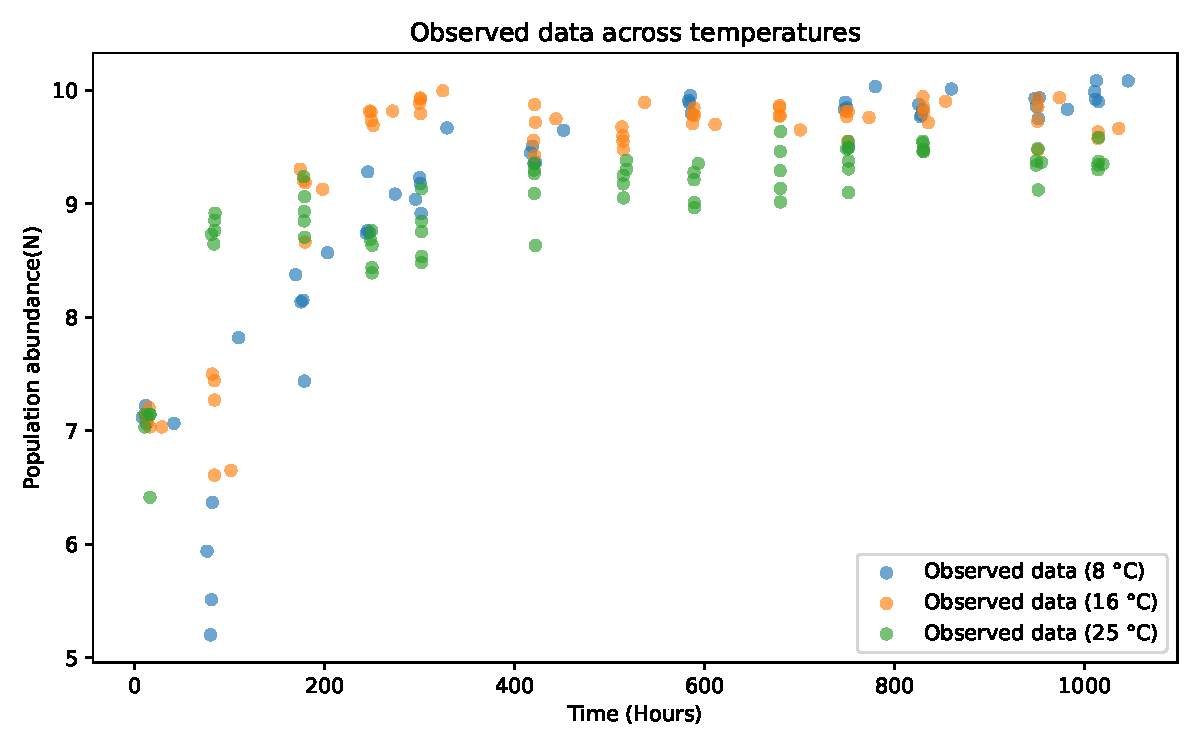
\includegraphics[width=0.6\textwidth]{fig/three_temperature_distribution.pdf}
    \caption{Observed data across temperatures.}
    \label{fig:three_temperature_distribution}
\end{figure}



\subsection{Growth models}

Three different of growth models were compared. The Logistic model, which describes growth as a continuous and smooth trajectory that rises gradually towards an upper asymptote through three quantities: carrying capacity, growth rate, and initial abundance; its principal advantage lies in its compact form and relative parsimony \cite{LOPEZ2004289}.

The Baranyi model has been used extensively in studies of microbial growth and whose main strength lies in incorporating the lag phase into the model structure itself, thereby making the delayed onset of growth easier to interpret as a biologically meaningful process than in the classical Logistic formulation\cite{BARANYI1994277}.

The third was the three-phase linear model, which divides growth explicitly into three stages: an initially near-flat lag phase, an approximately linear middle period of increase, and a later plateau in which the trajectory becomes level again; although this representation sacrifices some of the smoothness associated with continuous nonlinear curves, it does so in exchange for a structure in which phase boundaries are more visually transparent and biological interpretation correspondingly more direct\cite{BUCHANAN1997313}.

\subsection{Model fitting and comparison}
All models were fitted separately within each temperature condition. For each model, a multi start procedure was implemented.For each model, several fixed sets of initial values were fitted separately, and the fit associated with the lowest AIC was retained as the optimal model fit for subsequent analysis,which reduce the risk of convergence to a local optimum. Model performance was evaluated using $R^2$, RMSE, AIC, and BIC. Whereas $R^2$ and RMSE were used to summarise goodness of fit, AIC and BIC were used to compare models while accounting for differences in model complexity, and were therefore more informative for assessing whether additional model flexibility yielded sufficient gain in explanatory value. To facilitate a more direct examination of model behaviour under low-temperature conditions, the comparative results for all three models at $8^\circ$C were additionally summarised and presented in an overlaid fit plot.

\subsection{Computing tools}
A modular Python workflow was created for the analysis, consisting of separate scripts for dataset exploration,  preparation, model fitting, and final result comparison. Supporting packages included \texttt{pandas} for data handling, \texttt{numpy} for numerical computation, \texttt{matplotlib} for visualisation, \texttt{lmfit} for parameter handling and non-linear least squares(nlls) fitting, and \texttt{pathlib} for file and path management. Python was chosen because it provided a flexible working environment in which data preparation, model fitting, and result summarisation could be brought together more naturally, making the analysis easier not only to organise, but also to modify and extend as the workflow evolved.

\newpage
\section{Results}

All models were evaluated using both statistical criteria and visual inspection of the fitted curves, with model comparison based on AIC, together with $R^2$, RMSE and BIC.

At $8^\circ\mathrm{C}$, the models' ranking was unambiguous. Three-phase linear model gave the best overall fitting performance, Baranyi model followed closely, and the Logistic model performed worst. This pattern was reflected clearly in the AIC values, which were 61.59 for the three-phase linear model, 69.27 for the Baranyi model and 80.14 for the Logistic model. The curves also suggested that growth at $8^\circ\mathrm{C}$ retained a pronounced stage like structure.It has more apparent lag phase compared with three other temperature condition examined here. Which captured by three-phase linear and Baranyi models. The fitted results for the three models at $8^\circ\mathrm{C}$ are shown in Figure \ref{fig:comparison_at_8}, and the corresponding metrics are summarised in Table \ref{tab:model_metrics_all_temps}.

\begin{figure}[!ht]
    \centering
    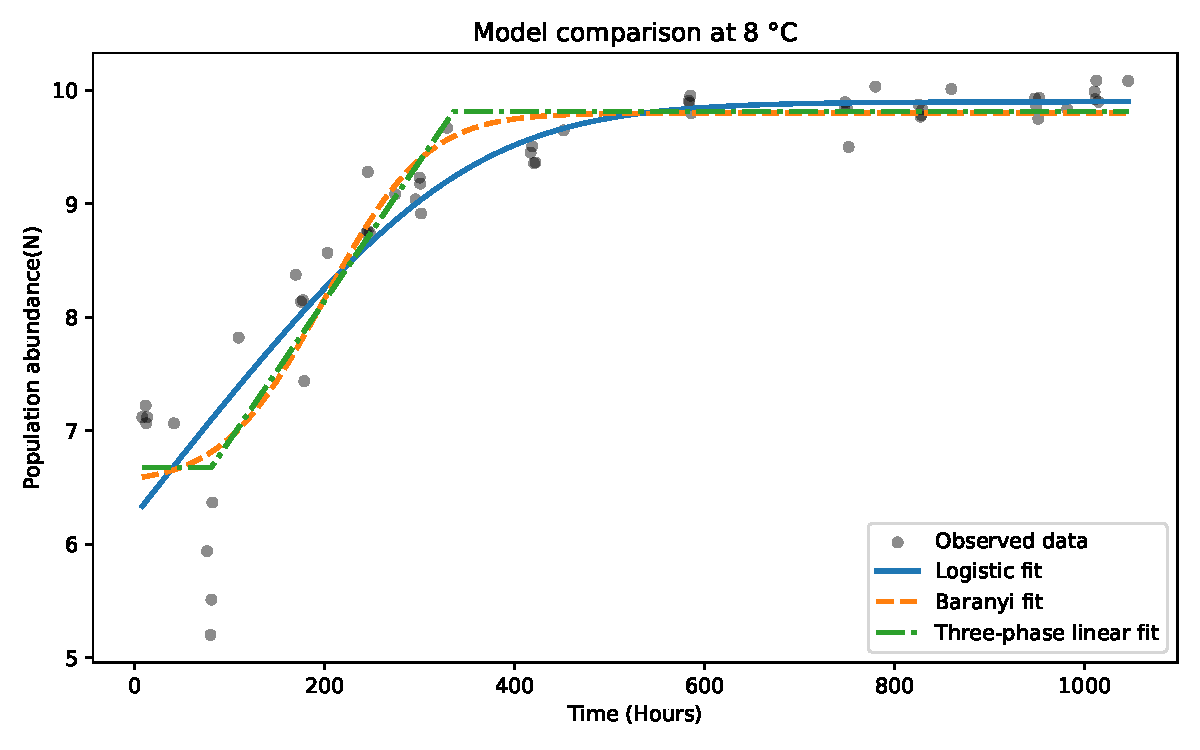
\includegraphics[width=0.6\textwidth]{fig/model_comparison_temp8.pdf}
    \caption{The data distribution and model fitting performance at $8^\circ\mathrm{C}$.}
    \label{fig:comparison_at_8}
\end{figure}

Under $16^\circ\mathrm{C}$ condition, three-phase linear model still maintained the lowest AIC ($-26.94$). Baranyi model close behind got a ($-25.40$) AIC; Logistic model once again performed worst among the three candidates, with an AIC of ($40.12$). Both the three-phase linear and Baranyi fits returned high $R^2$ and low RMSE(\ref{tab:model_metrics_all_temps}), their fitted curves were still able to resolve a clear lag phase. Logistic model still failed to capture a distinct lag phase. The fitted results at $16^\circ\mathrm{C}$ are shown in Figure~\ref{fig:comparison_at_16} and Table \ref{tab:model_metrics_all_temps}.

\begin{figure}[!ht]
    \centering
    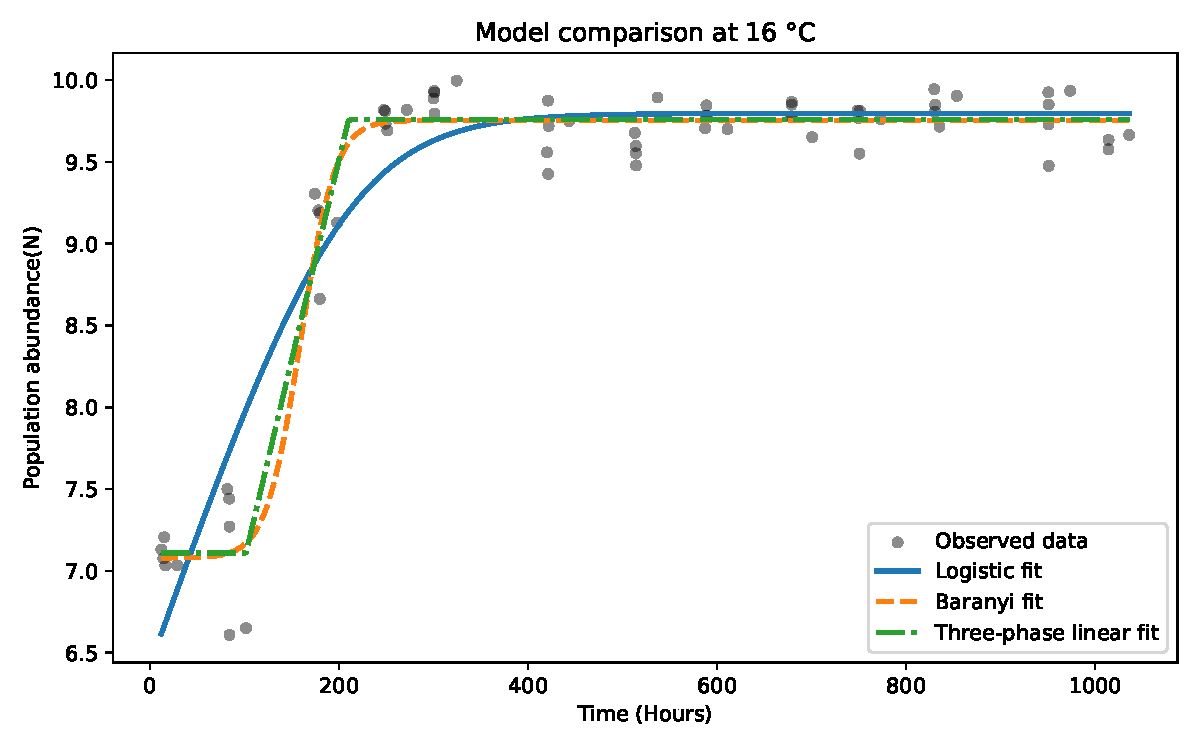
\includegraphics[width=0.6\textwidth]{fig/model_comparison_temp16.pdf}
    \caption{The data distribution and model fitting performance at $16^\circ\mathrm{C}$.}
    \label{fig:comparison_at_16}
\end{figure}



At $25^\circ\mathrm{C}$, the differences among models became much smaller. The Logistic model gave the lowest AIC ($38.01$), but the Baranyi ($38.88$) and three-phase linear ($38.86$) models were very close, indicating that the relative support for the three models was much less distinct than at the lower temperatures. Even so, the fitted curves still suggested a stage-like pattern in the data, and the lag phase appeared shortest at $25^\circ\mathrm{C}$. As at $8^\circ\mathrm{C}$, the Baranyi and three-phase linear models represented these growth stages more explicitly, while the Logistic model again failed to display a distinct lag phase.The fitted results of the three models at $8^\circ\mathrm{C}$ are shown in Figure \ref{fig:comparison_at_25}.

\begin{figure}[!ht]
    \centering
    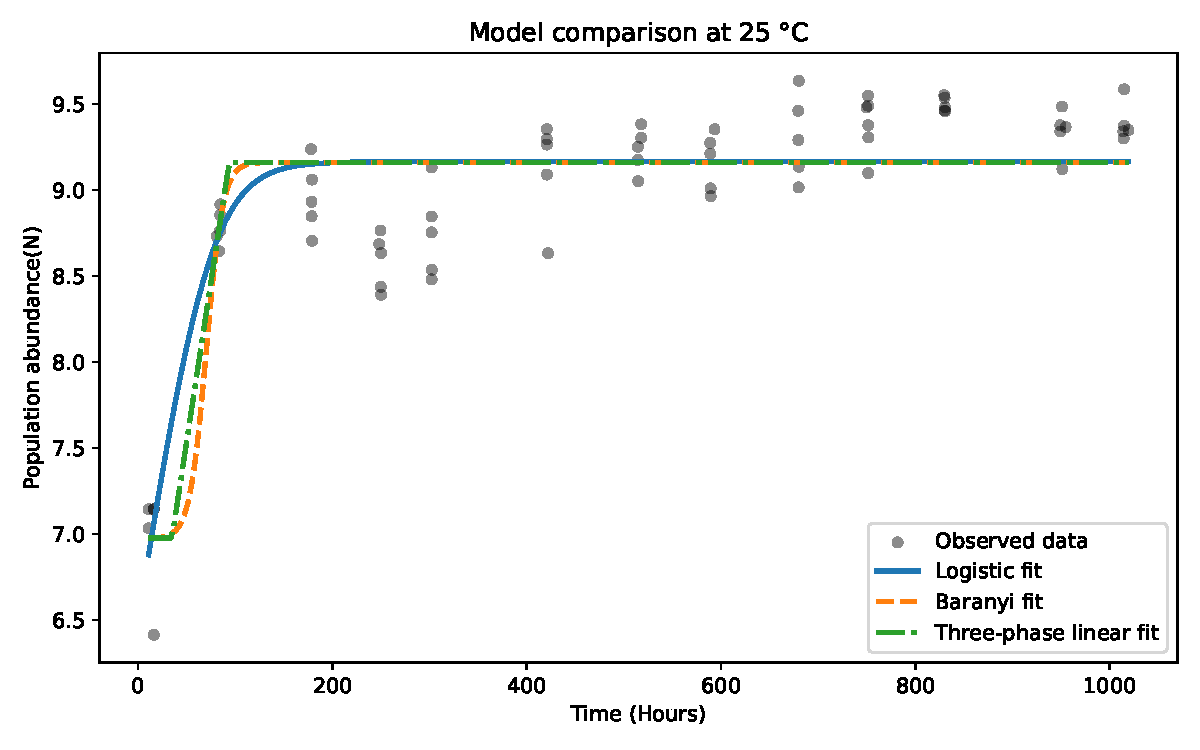
\includegraphics[width=0.6\textwidth]{fig/model_comparison_temp25.pdf}
    \caption{The data distribution and model fitting performance at $25^\circ\mathrm{C}$.}
    \label{fig:comparison_at_25}
\end{figure}
Detailed fitting results for the three models across different temperatures are presented in Table \ref{tab:model_metrics_all_temps}.

\newpage
The clearest overall statistical support was found at $16^\circ\mathrm{C}$, primarily on the basis of AIC, whereas the longest lag phase was observed at $8^\circ\mathrm{C}$ and the shortest at $25^\circ\mathrm{C}$. Across temperatures, the Baranyi and three-phase linear models generally captured phase-specific behaviour more effectively than the Logistic model.Both Table \ref{tab:model_metrics_all_temps} and the fitted curves shown above support the conclusion that the three-phase linear model outperformed the other two models for this dataset.

\begin{table}[!ht]
\centering
\caption{Model fitting metrics across temperatures for the three candidate models.}
\label{tab:model_metrics_all_temps}
\begin{tabular}{llccccc}
\hline
Model & Temp ($^\circ$C) & $R^2$ & RMSE & AIC & BIC \\
\hline
Baranyi & 8  & 0.8873 & 0.4267 & 69.2723  & 77.2282 \\
Logistic & 8  & 0.8570 & 0.4807 & 80.1434  & 86.1104  \\
Three-phase linear & 8  & 0.9022 & 0.3974 & 61.5924  & 69.5483 \\
\hline
Baranyi & 16 & 0.9642 & 0.1856 & -25.3999 & -16.8274  \\
Logistic & 16 & 0.8955 & 0.3172 & 40.1214  & 46.5508   \\
Three-phase linear & 16 & 0.9651 & 0.1834 & -26.9440 & -18.3715 \\
\hline
Baranyi & 25 & 0.7819 & 0.3057 & 38.8781  & 47.6367  \\
Logistic & 25 & 0.7781 & 0.3084 & 38.0150  & 44.5839  \\
Three-phase linear & 25 & 0.7819 & 0.3057 & 38.8572  & 47.6158  \\
\hline
\end{tabular}
\end{table}

\section{Discussion}
The aim of this study was to compare the ability of the three-phase linear, Baranyi and Logistic growth models to describe the population growth of \textit{Tetraselmis tetrahele} under a dataset of limited scale, with particular attention not only to their capacity to represent growth rates, but also to how effectively they could distinguish biologically growth phases. 

The results suggest that the advantage of the three-phase linear model was real, but also conditional rather than universal. At both $8^\circ\mathrm{C}$ and $16^\circ\mathrm{C}$, it provided the strongest overall performance among the three candidate models, with the distinction being especially marked at $8^\circ\mathrm{C}$, where it simultaneously achieved the highest $R^2$ and the lowest RMSE, AIC and BIC. By contrast, at $25^\circ\mathrm{C}$ the gap among models became much narrower: the three-phase linear and Baranyi models were almost indistinguishable in terms of fitting accuracy, while the Logistic model returned the lowest AIC and BIC. Taken together, these results indicate that the superiority of the three-phase linear model was most evident under low- and intermediate-temperature conditions, rather than being maintained to the same extent across all temperatures.


\section{Discussion}

The purpose of this study was not simply to identify which of three commonly used growth models could produce the lowest error for a single curve, but to examine, under a small and temperature-structured dataset, how consistently the three-phase linear, Baranyi and Logistic models could describe the growth trajectory of \textit{Tetraselmis tetrahele}, recover biologically interpretable changes in growth phase, and maintain a stable ranking across contrasting thermal conditions. In that sense, the present analysis was concerned as much with the \emph{shape} of the fitted trajectory as with goodness-of-fit in the narrow statistical sense. This distinction matters, because a model may provide an acceptable numerical fit while still failing to reflect the phase structure that gives microbial or population growth curves much of their biological meaning.

Several broad findings emerged clearly. All models were capable of fitting the observed trajectories to a reasonable degree, and none failed outright across all the temperature condition considered here. Quality of fit was strongest at $16^\circ\mathrm{C}$, which was supported by the corresponding values of $R^2$, RMSE,AIC and BIC(\ref{tab:model_metrics_all_temps}). At this condition, the three-phase linear model achieved the lowest AIC, followed by the Baranyi model, while the Logistic model was distinctly less well supported.Advantage of the three-phase linear model was not equally strong at all temperatures. Its superiority was most evident at $8^\circ\mathrm{C}$, where it simultaneously achieved the highest $R^2$ and the lowest RMSE, AIC and BIC. By contrast, at $25^\circ\mathrm{C}$ the gap among models became small; Logistic model returned the lowest AIC and BIC, while the Baranyi and three-phase linear models were almost indistinguishable. Thus, the main pattern is not one of unconditional dominance by a single model, but rather one in which model preference depends on temperature and, more importantly, on how distinctly the underlying growth stages are expressed in the data.

What emerges from the comparison is not simply that some models fit better than others, but that the three models differ quite fundamentally in how they are able to recognise growth phases in the first place. The Logistic model lacks direct mechanism for distinguishing or defined growth phases, therefore the least sensitive to phase separation, which cost failed to reveal the lag phase in any of the temperature conditions. The Baranyi model, by contrast, introduces lag phase at a more explicitly path ,a special  adjustment term, so that delayed population increase is treated as part of the model structure rather than as a by-product of curve itself. The three-phase linear model imposes this separation even more directly, since it forces the trajectory into three successive parts; an initial lag phase, a growth phase, and a plateau, with the transition points estimated from the data.For that reason, differences among models in this study are not only differences in statistical fit, but also differences in how clearly and accurately ecological information can be represented.

Lower temperatures generally prolong the period of physiological acclimation before sustained population growth begins, making the lag phase more visible. When that happens, the Baranyi and three-phase linear models are better able to capture the staged character of growth, and thus retain more ecological information about delayed activation and subsequent population increase. The Logistic model, in contrast, tends to smooth these transitions into a single continuous curve, which makes the phase structure less explicit\cite{NICOLA2019107563}.

In this respect, the present results sit comfortably within the broader modelling literature, in which statistical fit alone is seldom treated as sufficient grounds for model choice, and where models are often judged by a combination of goodness-of-fit, consistency across curves, and their capacity to recover biologically meaningful growth indicators \cite{LOPEZ2004289}. Similar results have also been reported at \cite{BUCHANAN1997313}, which also  support the view that the Baranyi and three-phase linear models tend to perform better. Although the present analysis is based on a far more limited dataset, the overall tendency was still apparent.Baranyi and three-phase linear models were better able to preserve visible phase, particularly at the lower and intermediate temperatures where lag transition remained evident.The better  performance of the three-phase linear model in this study is not especially surprising under a small and scale constrained dataset. Its simpler form may be better matched to the amount of information available and less likely to lose interpretability through unnecessary complexity.

The limitation of this study arises from the limited scale of the dataset itself. The dataset used here comprised fewer than 200 observations in total and was restricted to a single species and single medium. Although repeated measurements were available, but still should be regarded as a scale limited dataset rather than a broad comparative basis from which strong generalisations can safely be made. Conclusions drawn here should be interpreted with caution and should not be extended too readily beyond the specific experimental setting. The present comparison focused only on primary growth curves in log transformed abundance space and did not extend to a fuller residual based analysis of the kind used in broader model-evaluation studies, including assessments of serial correlation, accuracy factors and prediction bias \cite{LOPEZ2004289}. Future work based on a larger dataset spanning a wider temperature range, together with explicit comparisons at the replicate level and a more comprehensive residual analysis, would allow model choice to be evaluated in a more complete way, not only in terms of fit quality, but also with respect to robustness, bias and predictive stability.

Alternatively, one may argue that the range of modelling strategies considered here remains relatively narrow. The present comparison was restricted to three parametrised growth models with clear biological interpretation, and did not extend to more complex statistical or machine-learning frameworks, such as likelihood based approaches, neural networks or even deep learning methods. In principle, such methods may offer greater flexibility and may sometimes improve fit, especially when growth trajectories are irregular or when interactions among predictors become more complex. However, under a dataset of the present scale, they would likely face the same limitation of restricted information content and might even be more vulnerable to over fitting because of their higher effective model complexity. Approaches such as deep learning or neural networks usually involve much more parameters and often behave like black boxes, so may cost the lack of interpretability, added complexity, and greater risk of over fitting. In a dataset of this size, even routine strategies such as cross-validation or splitting the data into training and test sets would make an already limited dataset even thinner. As Buchanan et al. argued, a model is not necessarily better because it is more complex \cite{BUCHANAN1997313}.As shown by the performance of the three-phase linear model in the present study, a model can remain simple while still providing a very strong fit.

In conclusion, investigation suggest that the three-phase linear and Baranyi models should be preferred for describing \textit{Tetraselmis tetrahele} growth dataset.Both of them offered more convincing results. It also indicates that, under conditions of limited data scale, three-phase linear model may have better performance, as its relatively simple structure can still achieve strong fits while preserving sufficiently clear biological and ecological information.
\newpage

\bibliographystyle{apalike}
\bibliography{references}


\end{document}